% !TeX root = ../main.tex
\chapter{Extracting the multimodal fingerprint for transportation networks}

From bicycle paths to street and rail networks, mobility in cities increasingly relies on multimodality. These different modes of transportations can be conveniently described as multiplex networks, where layers are associated with different infrastructures. Here we show how to extract the multimodal blueprint of cities from their multiplex transportation networks. We identify clusters of cities with similar multimodal profiles, and link this feature to the level of sustainable mobility of each cluster. Our work highlights the importance of evaluating the transportation systems of a city altogether to correctly capture the nature of different urban clusters. 


\section{Prelude}
From a network perspective, the different modes of transportation can be described as a mathematical object, the multiplex transport network \cite{Morris2012,Strano2015,Aleta2017}. A city's multiplex transport network contains other network layers that have co-evolved with the street layer, such as the bicycle layer or the rail network layer, which together constitute the multimodal transportation backbone of a city. Due to the car-centric development of most cities \cite{Jacobs1961}, street layers are the most developed layers \cite{Gossling2016,Szell2018} and define or strongly limit other layers: For example, sidewalks are by definition footpaths along the side of a street and make up a substantial part of a city's pedestrian space \cite{Gossling2016}; similarly, most bicycle paths are part of a street or are built along the side. 

Here we consider the transport networks of 15 world cities and develop an urban fingerprinting technique based on multiplex network theory to characterize the various ways their transport layers are interconnected, outlining the potential for multimodal transport. Using clustering algorithms on the resulting urban fingerprints, we find clear classes of cities reflecting their transport priorities.

\section{METHODS AND DATA}
We acquired urban transportation networks from multiple cities around the world using OSMnx \cite{Boeing2017a}, a Python library to download and construct networks from OpenStreetMap (OSM). These data sets are of high quality \cite{Haklay2010b,Girres2010} in terms of correspondence with municipal open data \cite{Ferster2019} and completeness: More than $80\%$ of the world is covered by OSM \cite{Barbosa-Filho2017}.  The various analyzed urban areas and their properties are reported in Table~\ref{tab:Table1}. Figure \ref{fig:fig01} shows the different network layers for two of our analyzed cities. The pedestrian layer contains all sidewalks and pedestrian paths. The bicycle layer consists of all infrastructure exclusive to bicycles, like designated cycleways and bicycle trails. The rail network captures all public transportation that uses rails, including subways and tramways. Finally, the street layer is composed of all streets designated for motor vehicles.

\begin{table*}[ht!]
	\centering
	\begin{adjustbox}{width=0.6\textwidth,keepaspectratio}
		\begin{tabular}{lrrrrrrrrl}
			\toprule
			{} & \multicolumn{2}{l}{walk} & \multicolumn{2}{l}{bike} & \multicolumn{2}{l}{rail} & \multicolumn{2}{l}{drive} &  Population \\
			{} &     $N$ & $CC$ &    $N$ &  $CC$ &   $N$ & $CC$ &     $N$ & \multicolumn{2}{l}{$CC$} \\
			\midrule
			Amsterdam  &   23321 &    1 &  34529 &   355 &  1096 &    8 &   15125 &    1 &     872,680 \\
			Barcelona  &   20203 &    1 &   7553 &   122 &   249 &   15 &   10393 &    1 &   1,600,000 \\
			Bogota     &   81814 &    1 &   9760 &   171 &   166 &   12 &   62017 &    1 &   7,412,566 \\
			Budapest   &   73172 &    1 &  10494 &   257 &  1588 &   20 &   37012 &    1 &   1,752,286 \\
			Copenhagen &   30746 &    1 &  13980 &   321 &   276 &    3 &   15822 &    1 &   2,557,737 \\
			Detroit    &   47828 &    1 &   3663 &    53 &    20 &    3 &   28462 &    1 &     672,662 \\
			Jakarta    &  140042 &    1 &    248 &    19 &    58 &    6 &  138388 &    1 &  10,075,310 \\
			LA         &   89543 &    1 &  14577 &   230 &   173 &    9 &   71091 &    1 &   3,792,621 \\
			London     &  270659 &    1 &  62398 &  3023 &  2988 &   38 &  179782 &    1 &   8,908,081 \\
			Manhattan  &   13326 &    1 &   3871 &   105 &   349 &    5 &    5671 &    1 &   1,628,701 \\
			Mexico     &  108033 &    1 &   5218 &    52 &   370 &   17 &   95375 &    1 &   8,918,653 \\
			Phoenix    &  111363 &    1 &  35631 &   141 &   105 &    4 &   73688 &    1 &   1,445,632 \\
			Portland   &   50878 &    1 &  24252 &   198 &   230 &    2 &   35025 &    1 &     583,776 \\
			Singapore  &   82808 &    1 &  12981 &   104 &   683 &   14 &   50403 &    1 &   5,638,700 \\
			\bottomrule
			\end{tabular}
	\end{adjustbox}
	\caption{Measures for the administrative area of analyzed cities. The number of connected components ($CC$) and nodes ($N$) for each layer in all cities of our dataset are highly diverse due to the varying developmental levels and focus of transport. 
		\label{tab:Table1}}
\end{table*}

The codes to replicate the results are available as Jupyter Notebooks in: (\url{https://github.com/nateraluis/bicycle-network-growth}), and the data can be downloaded from Harvard Dataverse (\url{https://doi.org/10.7910/DVN/GSOPCK})

We characterize each city as a multiplex network \cite{Boccaletti2014,Kivela2014,Battiston2017a} with $M$ layers and $N$ nodes that can be active in one or more layers in the system. Layers are represented by a primal approach \cite{Porta2006} in which nodes are intersections (that may be present in one or more layers), while links represent streets (s), bicycle paths and designated bicycle infrastructure (b), subways, trams and rail infrastructure (r), or pedestrian infrastructure (p). This recent approach has been useful to demonstrate how cities grow \cite{Strano2012,Barthelemy2013}, how efficient \cite{Gallotti2014} and dense they are, and to capture the tendency of travel routes to gravitate towards city centers \cite{Lee2017}. Each layer $\alpha=1, \dots, M$ is described by an adjacency matrix $A^{[\alpha]}=\{a_{ij}^{[\alpha]}\}$ where $a_{ij}^{[\alpha]}=1$ if there is a link between nodes $i$ and $j$ in layer $\alpha$ and 0 otherwise. The multiplex urban system is then specified as a vector of adjacency matrices $\textbf{A} = (A^{[1]}, \ldots, A^{[M]})$.


\begin{figure*}[t!]
	\centering
	\includegraphics[width=\textwidth]{images/multiplex/Fig01.png}
	\caption{{\textbf (Map plots, left)} Networks representing various layers of transport infrastructure (pedestrian paths, bicycle paths, rail lines, and streets) for  Copenhagen and London, with data from OpenStreetMap. {\textbf (Right)} Connected component size distribution $P(N_{cc})$ as a function of the ranking of the component for all considered network layers and cities. All layers are well connected except the bicycle layer: Copenhagen has 321 bicycle network components despite being known as a bicycle-friendly city, while London's bicycle layer is much more fragmented, featuring over 3000 disconnected components. Copenhagen's largest connected bicycle component (leftmost data point) spans 50\% of the network, but London's only less than 5\%.}
	\label{fig:fig01}
\end{figure*}

\section{FINDINGS}
In a multimodal city, we expect to find many transport hubs that connect different layers, such as train stations with bicycle and street access, i.e. nodes that are active in different multiplex configurations. Note that even in a multimodally ''optimal'' city there will be a high heterogeneity of node activities due to the different speeds and nature of transport modes, implying, for example, a much lower density of nodes necessary for a train network than for a bicycle network. Here we build a way to see and compare all combinations of node activities in the system, that help us learn how much focus a city puts on connecting different modes. We can define such a fingerprint using the multiplex network formalism. We call the plot that counts the combinations of node activities a city's \emph{overlap census} (Figure \ref{fig:fig02}). Similar to edge overlap \cite{Bianconi2013,Battiston2014a} and multiplex motifs \cite{Battiston2017} that provide a characterization of multiplexity at the local scale, the overlap census captures the percentage of nodes that are active in different multiplex configurations and provides an "urban fingerprint'' of multimodality \cite{Aleta2017}.

\begin{figure*}[t!]
	\centering
	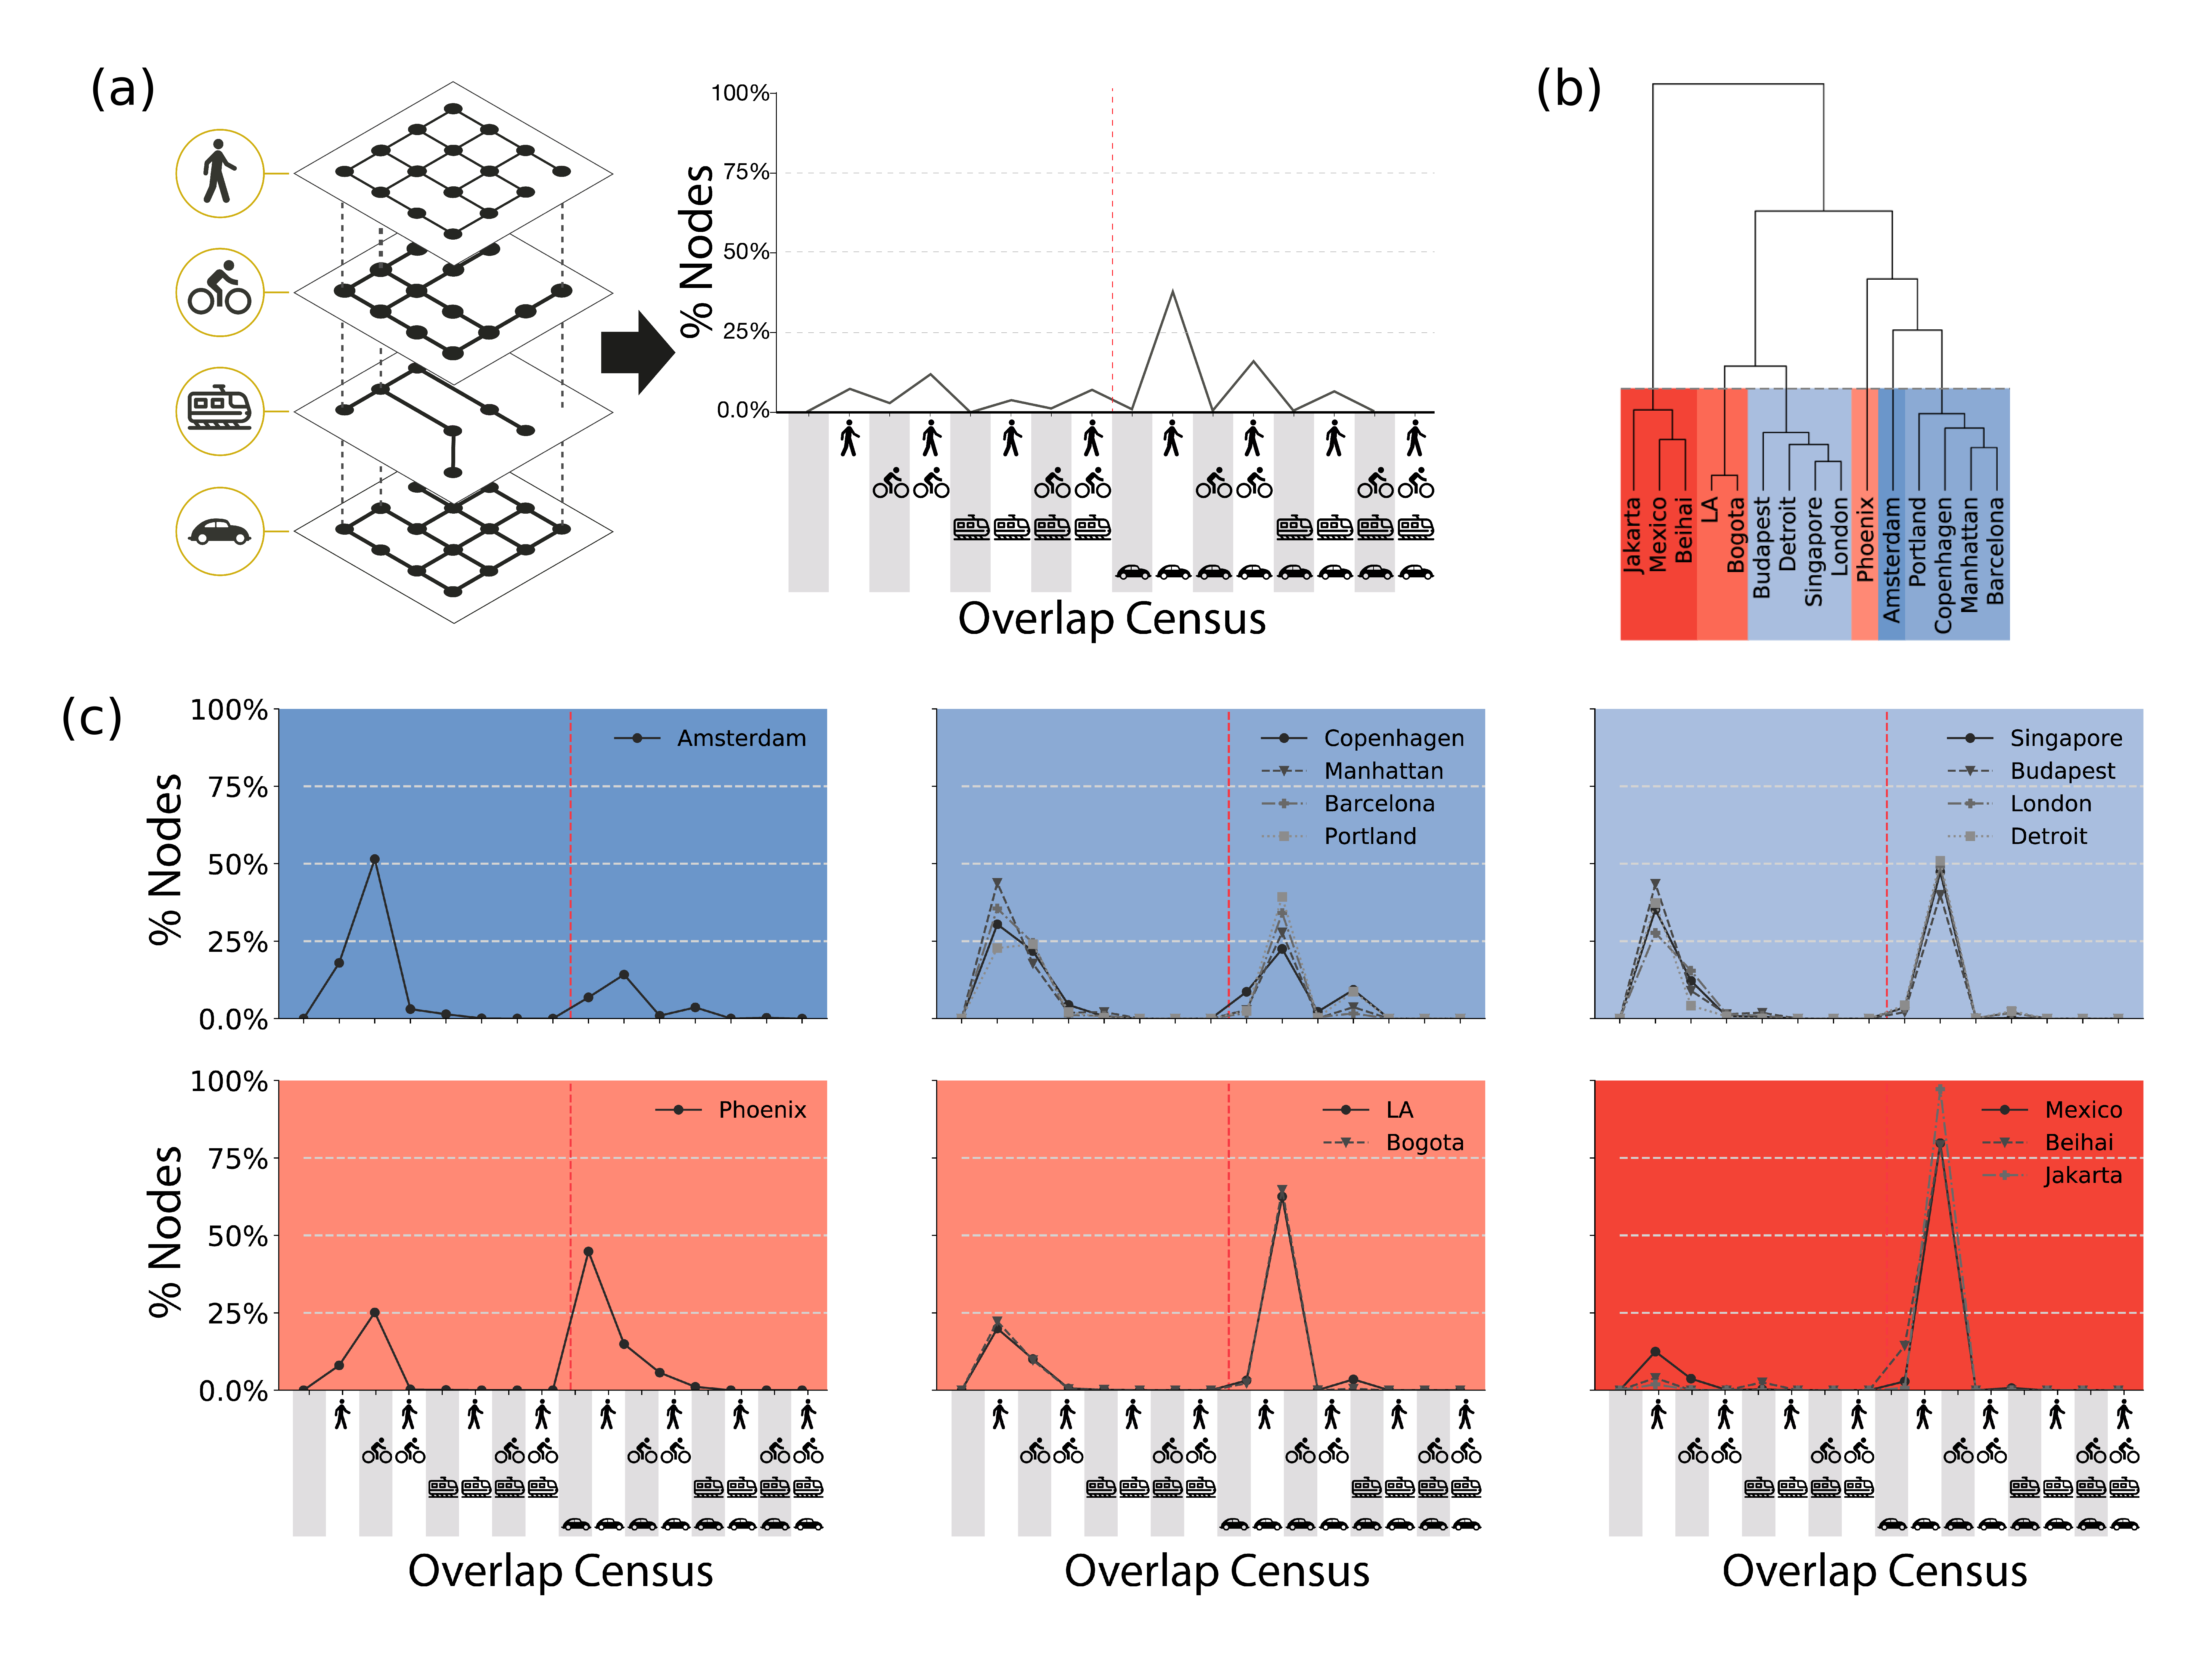
\includegraphics[width=0.8\textwidth]{images/multiplex/Fig02.png}
	\caption{
		\textbf{(a)} Schematic of multiplex layers in a city (left) and its transformation to the overlap census (right). In the overlap census, the vertical red line gives a visual separation of the left from the right half where nodes become active in the street layer. High spikes in the right half indicate car-centricity.
		 \textbf{(b)} Clusters of cities based on similarity of their overlap census. We find six different clusters using a k-means algorithm (coloured areas), which explain more than $90\%$ of the variance.
		 \textbf{(c)} Overlap census for cities in each cluster. The first one corresponds to Amsterdam (the city with most active nodes in bicycle-only configurations). The Copenhagen-Manhattan-Barcelona-Portland city cluster has many active nodes in pedestrian-only and bicycle-only configurations, representing an active mobility city. The clusters of Los Angeles-Bogota and Mexico-Beihai-Jakarta are car-centric.}
	\label{fig:fig02}
\end{figure*}

To define the overlap census formally, we calculate the degree of each node in layer $\alpha$ as $ k_i^{[\alpha]}=\sum_ja_{ij}^{[\alpha]} $. We store degrees in a vector for each layer, \textbf{\textit{k}}$^{[\alpha]}=(k_i^{[\alpha]}, \dots, k_n^{[\alpha]})$, indicating layers by `p' for pedestrian, `b' for bicycle, `r' for rail infrastructure, and `s' for streets, as before. The use of vectorial variables like \textbf{A} and \textbf{\textit{k}}$^{[\alpha]}$ instead of those of the aggregated network lets us capture the richness of the system and work in the various layers independently. Given a Multiplex transport network with $M$ layers the overlap census is a vector of $2^{M-1}$ components, which accounts for the fractions of nodes that can be reached through at least one layer.

In Fig.~\ref{fig:fig02}(a) we show a schematic of how the overlap census is built: taking the multiplex network, transforming it to its corresponding degree vectors for all layers in the system, and calculating the percentage of nodes that overlap in different configurations. Note that the overlap census provides more information than a simple counting of nodes, edges, or other single-layer network measures. The multiplex approach addresses the multimodality of a city: it not only counts how many nodes or links there are in each layer, but it shows how they are combined, revealing the possible multimodal mobility combinations in the city. Understanding the possibilities for interchange between mobility layers provides us with a better understanding of urban systems, showing us the complexity and interplay between layers.

A good way to assess a city's overlap census is by comparing it with the overlap census of other cities. Explicitly, we find similarities between cities via a k-means algorithm. The algorithm separates the 15 analyzed cities into six different clusters [Fig.~\ref{fig:fig02}(b)]. On the left half of the overlap census, we show the configurations in which nodes are not active in the street layer, while the right half contains car-related configurations. These clusters of cities are useful to explain similarities in infrastructure planning in different urban transport development paths \cite{Rodrigue2013,Louf2014}, with clusters of car-centric urbanization (like Mexico, Beihai, and Jakarta) opposed to clusters that show a more multimodally focused evolution of their urban mobility infrastructure (like Copenhagen, Manhattan, Barcelona, and Portland). In the extreme cluster that contains only Amsterdam, close to $50\%$ of nodes are active in the bicycle layer, while in the Mexico-Beihai-Jakarta cluster more than $50\%$ of nodes are active in the street-pedestrian configuration. This concentration of nodes in just one configuration informs us not only about the (sometimes already well-known) mobility character of the city, i.e. Amsterdam being a bicycle-friendly city, but unveils the importance of explicitly considering overlooked layers and their interconnections. For example, Singapore, Budapest, London, and Detroit have two main peaks indicating that most of their nodes are either active in the street-pedestrian or only in the pedestrian configuration, i.e. there are plenty of walkable areas exclusive to pedestrians. This is not the case in Los Angeles and Bogota, where the majority of nodes are active in the car-pedestrian combination, i.e. the pedestrians have to share most of the city with cars.